\documentclass[../Thesis.tex]{subfiles}
\graphicspath{{\subfix{../figures/}}}
% \epstopdfsetup{outdir={../figures/}}
\usepackage{xr}
\externaldocument{C4 Method}
\externaldocument{../_BackMatter/Appendix1}
\begin{document}

\chapter{Results}
\section{Examples}
In this section, we will investigate how the algorithms \autoref{alg:Gobs1} and \autoref{alg:ND} works in junction and, if so, observe how the algorithm can fail and what may be done to correct such cases. Initially, a few simple examples involving exponentiated multivariate Gaussians $\boldsymbol Y $.

\subsection{Gaussian CE error}\label{sec:gaussian MI error}
\textcolor{red}{Eksempel medd normal fordeling og fejlen der bliver lavet vha. algoritmen.}
\begin{proposition} \label{prop:MI bivariate gaussian}
    Given a bivariate normal distribution $\boldsymbol X \sim \mathcal{N}\left(\boldsymbol \mu,  \Sigma\right)$ where
    $$\Sigma =
        \begin{bmatrix}
            \sigma_1^2             & \rho \sigma_1 \sigma^2 \\
            \rho \sigma_1 \sigma_2 & \sigma_2^2
        \end{bmatrix}
    $$
    Then the mutual information $I\left(X_1, X_2\right) = -\frac{1}{2}\ln \left(1 - \rho^2\right)$.
\end{proposition}
\begin{proof}
    This follows by direct computation Using e.g. that $I(X_1, X_2) = h(X_1) + h(X_2) - h(X_1, X_2)$
\end{proof}

\begin{example} \label{ex:1}
    Exponentiated multivariate Gaussian

    Let us consider a simple case with $\mathbf{Y} = e^{\mathbf{X}}$ (element wise exponentiation) where $X \sim \mathcal{N}\left(\mathbf{0}, \Sigma\right)$ where
    $$\Sigma = \begin{bmatrix}
            \sigma_1^2           & 0.9\sigma_1\sigma_2 & 0          \\
            0.9 \sigma_1\sigma_2 & \sigma_2^2          & 0          \\
            0                    & 0                   & \sigma_3^2
        \end{bmatrix}$$
    It is clear that to \autoref{alg:Gobs1}, the mean is of no importance as it simply corresponds to a scaling of the $Y_i$ variables. Furthermore, because of \autoref{coro: Coordinate transformation}, theoretically, due to the uniqueness of the Copula $C$ (as $\boldsymbol Y$ is continuous) we should expect near equal or very similar results for $\boldsymbol Y$ and $\boldsymbol X$ from \autoref{alg:Gobs1}. Additionally, different $\sigma$ corresponds to different scaling of $\boldsymbol X$, and thus we should observe equal or near equal $G_{dir}$ for all $\boldsymbol Y$. Initially, we shall see how this hypothesis holds up to the following three examples
    $$
        \boldsymbol\sigma = (0.07, 0.3, 0.9), \quad
        \boldsymbol\sigma = (1,1,1), \quad
        \boldsymbol\sigma = (1,2,3)
    $$
    In order for the sample size to not influence the results, we simulate a generous number of samples, namely, for the following results we have used $n = 10{,}000$ samples. For $\boldsymbol\sigma = (1,1,1)$, \autoref{alg:Gobs1} and \autoref{alg:ND} returns the following (using $\alpha = 1$ and $\beta = 0.99$)
    \begin{equation} \label{eq:s medium G_dir}
        G_{dir} =
        \begin{bmatrix}
            -0.33396 & 0.6660  & 0.02512    \\
            0.6660   & -0.3341 & 0.02730    \\
            0.02512  & 0.02730 & -0.0020583
        \end{bmatrix}
    \end{equation}
    Similarly, for $\boldsymbol\sigma = (0.07, 0.3, 0.9)$:
    \begin{equation} \label{eq:s small G_dir}
        G_{dir} =
        \begin{bmatrix}
            -0.3335 & 0.6665  & 0.01414     \\
            0.6665  & -0.3335 & 0.01418     \\
            0.01414 & 0.01418 & -0.00060124
        \end{bmatrix}
    \end{equation}
    Finally, for $\boldsymbol\sigma = (1,2,3)$:
    $$ G_{dir} =
        \begin{bmatrix}
            -0.1490 & 0.09535 & 0.3599  \\
            0.09535 & -0.2989 & 0.5831  \\
            0.3599  & 0.5831  & -0.4037
        \end{bmatrix}
    $$
    For $\boldsymbol\sigma = (1,1,1)$ and $\boldsymbol\sigma = (0.07, 0.3, 0.9)$ we observe the most resemblance to the $\Sigma$, although the resulting $G_{dir}$ deviate in the final column. The difference is likely produced by \autoref{alg:Gobs1} as if the resulting $G_{obs}$ was the same, then so would $G_{dir}$ and from the above argument, we know that theoretically this should be the case. For the final example, $\boldsymbol\sigma = (1,2,3)$, we see a completely different result and immediately suspect that there must be some numerical errors. Investigating the partial results of \autoref{alg:Gobs1} we immediately see a flaw in the supposedly uniform variables $U_i$ as shown in figure \autoref{fig:Gaussian 3x3 large s uniforms}
    \begin{figure}[H]
        \centering
        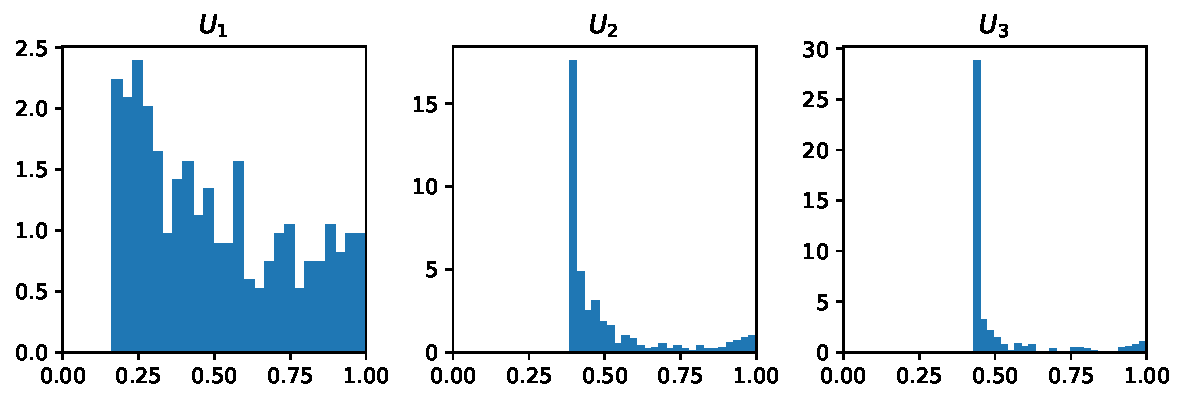
\includegraphics[width=0.99\linewidth]{figures/ND examples/Gaussian 3x3 large s uniforms.pdf}
        \caption{The samples transformed using $U_i = F_i(X_i)$ for $\boldsymbol\sigma = (1,2,3)$. These should be uniformly distributed, but clearly this is not the case for $U_2$ and $U_3$. Even $U_1$ does not quite resemble $10{,}000$ samples from a uniform distribution.}
        \label{fig:Gaussian 3x3 large s uniforms}
    \end{figure}
    \begin{table}[h]
        \centering
        \begin{tabular}{c|c|c|c}
                    & $U_1$    & $U_2$   & $U_3$   \\\hline
            $D_n$   & 0.066209 & 0.36014 & 0.46285 \\
            p-value & 0        & 0       & 0
        \end{tabular}
        \caption{based on 10,000 samples for $\boldsymbol\sigma = (1, 2, 3)$.}
    \end{table}
    Before handling this, the non-uniformity of $U_1$ in \autoref{fig:Gaussian 3x3 large s uniforms} is likely also present in the case when $\boldsymbol\sigma = (1,1,1)$. Indeed, \autoref{fig:Gaussian 3x3 medium s uniforms} shows that this is indeed the case.
    \begin{figure}[H]
        \centering
        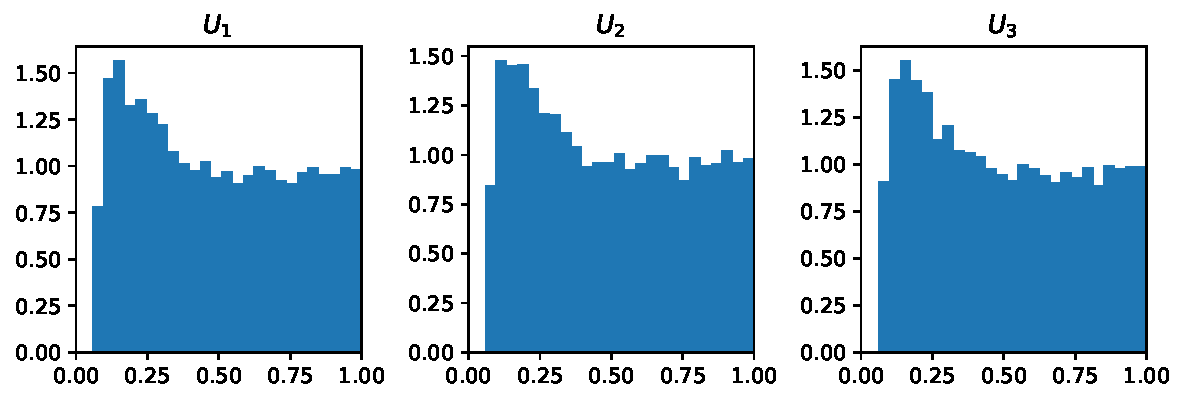
\includegraphics[width=0.99\linewidth]{figures/ND examples/Gaussian 3x3 medium s uniforms.pdf}
        \caption{The samples transformed using $U_i = F_i(X_i)$ for $\boldsymbol\sigma = (1,1,1)$.}
        \label{fig:Gaussian 3x3 medium s uniforms}
    \end{figure}
    \begin{table}[h]
        \centering
        \begin{tabular}{c|c|c|c}
                    & $U_1$    & $U_2$    & $U_3$    \\\hline
            $D_n$   & 0.068408 & 0.066808 & 0.070809 \\
            p-value & 0        & 0        & 0
        \end{tabular}
        \caption{based on 10,000 samples for $\boldsymbol\sigma = (1, 1, 1)$.}
    \end{table}
    Finally, just to be sure, $\boldsymbol\sigma = (0.07, 0.3, 0.9)$ is also shown in \autoref{fig:Gaussian 3x3 small s uniforms} and seems very reasonable, except for $U_3$.
    \begin{figure}[H]
        \centering
        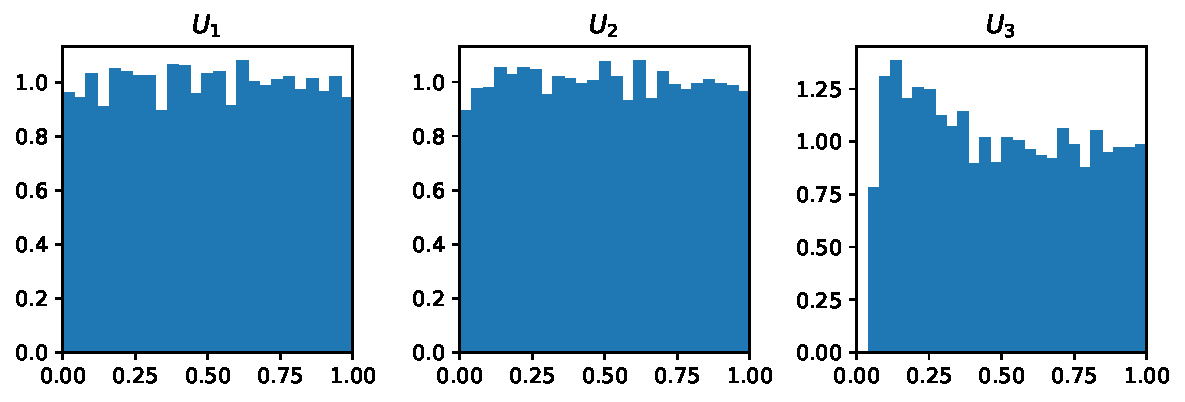
\includegraphics[width=0.99\linewidth]{figures/ND examples/Gaussian 3x3 small s uniforms.pdf}
        \caption{\raggedright The samples transformed using $U_i = F_i(X_i)$ for $\boldsymbol\sigma = (0.07, 0.3, 0.9)$.\hfill}
        \label{fig:Gaussian 3x3 small s uniforms}
    \end{figure}
    \begin{table}[h]
        \centering
        \begin{tabular}{c|c|c|c}
                    & $U_1$      & $U_2$     & $U_3$    \\\hline
            $D_n$   & 0.00581897 & 0.0068066 & 0.050908 \\
            p-value & 0.88645    & 0.74179   & 0
        \end{tabular}
        \caption{based on 10,000 samples for $\boldsymbol\sigma = (0.07, 0.3, 0.9)$.}
    \end{table}
    From the above examples, it seems that the larger the variance, the worse the uniforms turn out. Reasons for this could include numerical issues when trying to calculate $u_i^{(j)}$ form $y_i^{(j)}$ by $u_i^{(j)} = \int_{-\infty}^{y_i^{(j)}} f_i(y) \, dy$ and bad fitting of the kernel density estimate from observations. In particular, for values similar, which happens in the case for large $\sigma$ such that we observe large negative realizations of $X_i$, $y_i^{(j)}$ are almost 0, and when computing the integral could result in identical values. Furthermore, from \autoref{fig:Gaussian 3x3 large s X3 KDE} we see that indeed the fit is quite poor. Note that we have zoomed in on the interval $[-200 , 200]$ which contains $96.2\%$ of observations. The poor fit is primarily due to the use of Scott's Rule \textcolor{red}{as discussed above} which in this case overshoots the optimal bandwidth by a lot.
    \begin{figure}[H]
        \centering
        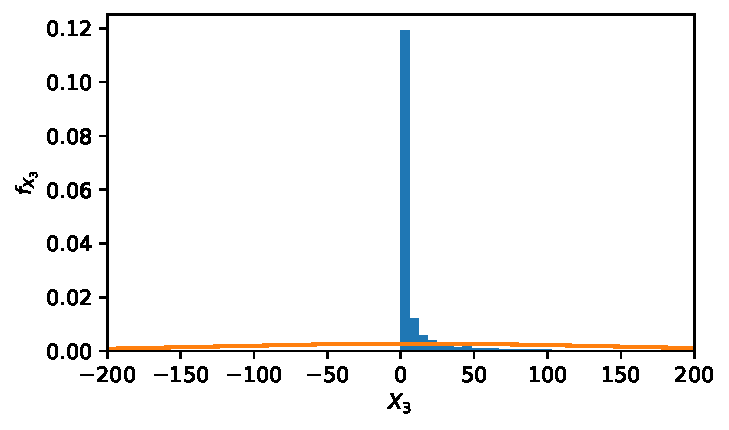
\includegraphics[width=0.7\linewidth]{figures/ND examples/Gaussian 3x3 large s X3 KDE.pdf}
        \caption{}
        \label{fig:Gaussian 3x3 large s X3 KDE}
    \end{figure}
    The poor fit also explains the high concentration of $U_3$ around $0.5$ in \autoref{fig:Gaussian 3x3 large s uniforms} as only $54.5\%$ of the probability mass lies above $0$.

    However, also here \autoref{coro: Coordinate transformation} proves to be useful. Namely, we can get rid of the numerical issues by transforming $Y_i$ using e.g. $\log(\cdot)$ or $(\cdot)^{p}$ for $p>0$ to get even out the observations more. As the first simply inverts the initial transformation of $X_i$, we choose the latter as a more interesting case. In particular, choosing $p<1$ will result in a more even distribution. In the following, $p=1/10$ has been used to transform $\boldsymbol Y$ prior to running \autoref{alg:Gobs1} and the resulting $u_i^{(j)}$ is shown in \autoref{fig:Gaussian 3x3 large s power uniforms}.
    \begin{figure}[H]
        \centering
        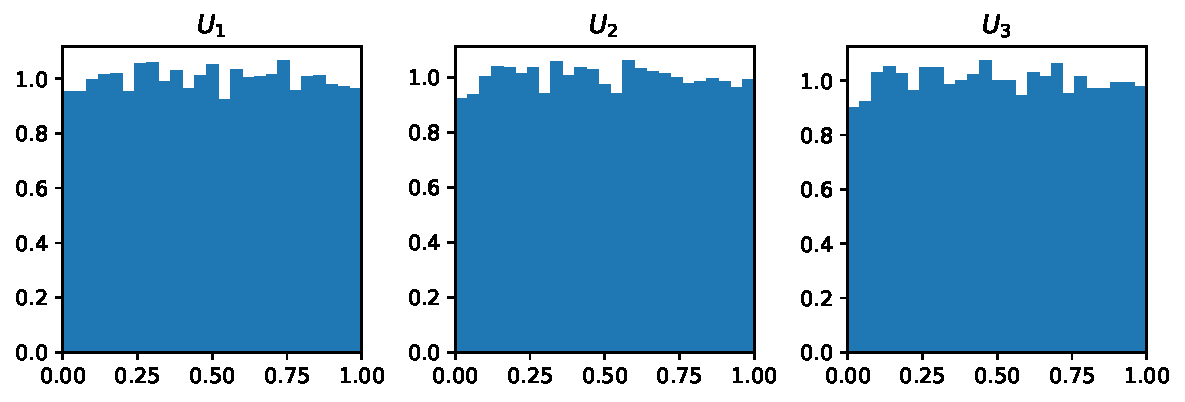
\includegraphics[width=0.99\linewidth]{figures/ND examples/Gaussian 3x3 large s power uniforms.pdf}
        \caption{}
        \label{fig:Gaussian 3x3 large s power uniforms}
    \end{figure}
    \begin{table}[h]
        \centering
        \begin{tabular}{c|c|c|c}
                    & $U_1$     & $U_2$     & $U_3$     \\\hline
            $D_n$   & 0.0061099 & 0.0061435 & 0.0073148 \\
            p-value & 0.84838   & 0.84368   & 0.65690
        \end{tabular}
        \caption{based on 10,000 samples for $\boldsymbol\sigma = (1, 2, 3)$ with power transform.}
    \end{table}
    The resulting $u_i^{(j)}$ now seem to follow a uniform distribution and indeed the KDE fits much better as seen in \autoref{fig:Gaussian 3x3 large s power X3 KDE}.
    \begin{figure}[H]
        \centering
        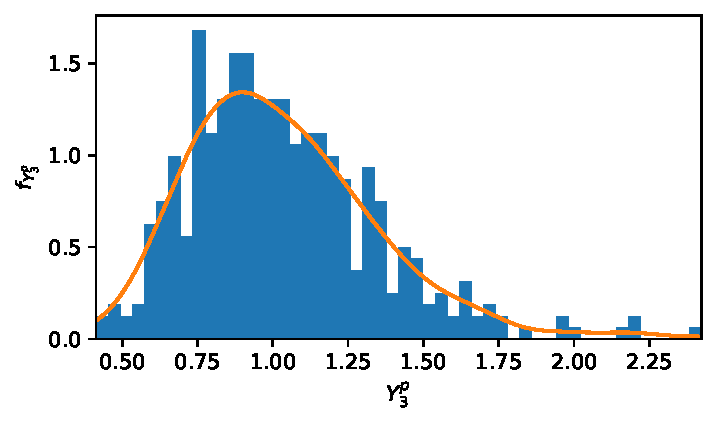
\includegraphics[width=0.7\linewidth]{figures/ND examples/Gaussian 3x3 large s power X3 KDE.pdf}
        \caption{}
        \label{fig:Gaussian 3x3 large s power X3 KDE}
    \end{figure}
    Turning to \autoref{alg:Gobs1} and \autoref{alg:ND} we now find that $G_{dir}$ is given by
    $$G_{dir} =
        \begin{bmatrix}
            -0.3290  & 0.6610   & 0.008440   \\
            0.6610   & -0.3290  & 0.008150   \\
            0.008440 & 0.008150 & -0.0002061
        \end{bmatrix}
    $$
    Which is indeed much more comparable with the result from before in \autoref{eq:s medium G_dir} and \autoref{eq:s small G_dir}. The difference between $G_{dir}$ from $\boldsymbol Y$ and $\boldsymbol Y^p$ is clearly visible in \autoref{fig:Gaussian 3x3 large s G_dir differences} and also \autoref{fig:Gaussian 3x3 large s power} resembles the original correlation structure.
    \begin{figure}[H]
        \centering
        \begin{subfigure}[t]{0.49\textwidth}
            \centering
            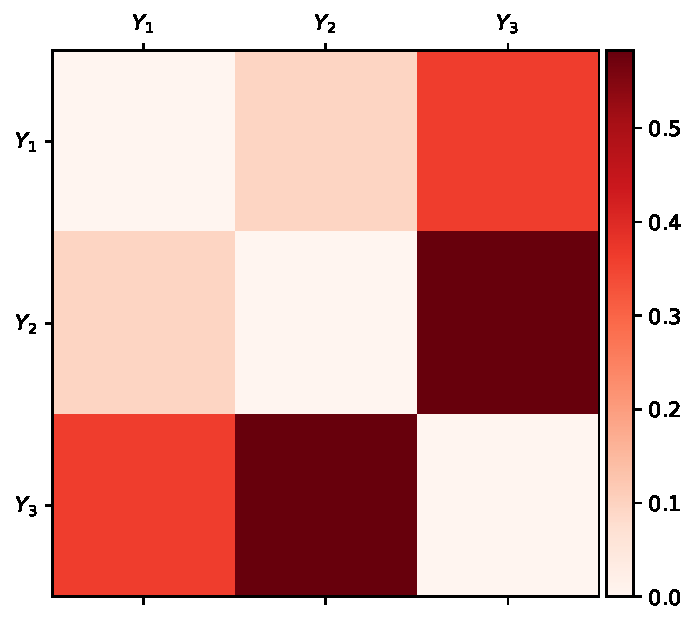
\includegraphics[width=\linewidth]{figures/ND examples/Gaussian 3x3 large s.pdf}
            \caption{}
            \label{fig:Gaussian 3x3 large s}
        \end{subfigure}%
        ~
        \begin{subfigure}[t]{0.49\textwidth}
            \centering
            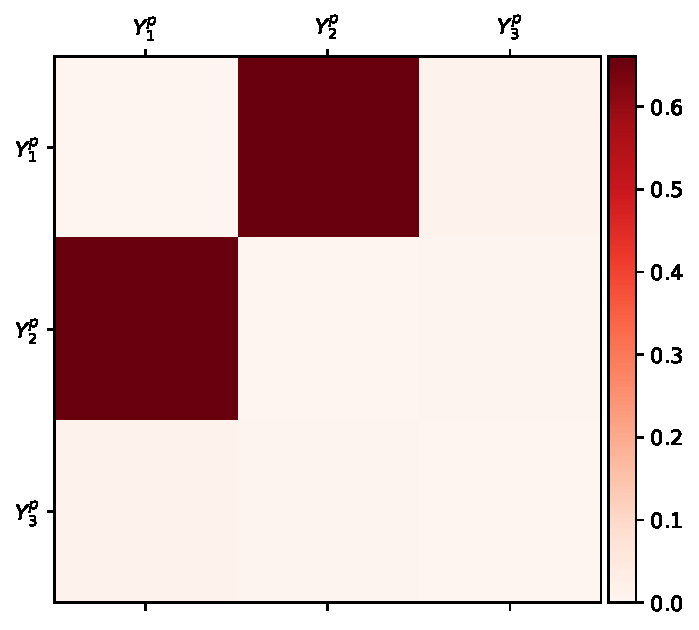
\includegraphics[width=\linewidth]{figures/ND examples/Gaussian 3x3 large s power.pdf}
            \caption{}
            \label{fig:Gaussian 3x3 large s power}
        \end{subfigure}
        \caption{$G_{dir}$ resulting from $10{,}000$ samples from multi variate Gaussian with $\boldsymbol\sigma = (1,2,3)$ in \textbf{(a)} with raw samples from $\boldsymbol Y$ and in \textbf{(b)} the transformed data corresponding to $\boldsymbol Y^p$.}
        \label{fig:Gaussian 3x3 large s G_dir differences}
    \end{figure}
    Finally, to end this example we shall compare with some theoretical results. Namely, the output $G_{obs}$ of \autoref{alg:Gobs1} can also be calculated theoretically. For this, we shall use \autoref{prop:MI bivariate gaussian} which permits a theoretical result, namely
    \begin{align*}
        G_{obs} & =
        \begin{bmatrix}
            0                                              & -\frac{1}{2} \ln \left( 1 - \rho_{12}^2\right) & -\frac{1}{2} \ln \left( 1 - \rho_{13}^2\right) \\
            -\frac{1}{2} \ln \left( 1 - \rho_{21}^2\right) & 0                                              & -\frac{1}{2} \ln \left( 1 - \rho_{23}^2\right) \\
            -\frac{1}{2} \ln \left( 1 - \rho_{31}^2\right) & -\frac{1}{2} \ln \left( 1 - \rho_{32}^2\right) & 0
        \end{bmatrix} \\
                & \cong
        \begin{bmatrix}
            0       & 0.83037 & 0 \\
            0.83037 & 0       & 0 \\
            0       & 0       & 0
        \end{bmatrix}
    \end{align*}
    Similarly, prior to deconvolution, using just the sampled $\boldsymbol X$ (i.e. no exponential transform), \autoref{alg:Gobs1} returns
    $$G_{obs} =
        \begin{bmatrix}
            0.         & 0.71841756 & 0.01781815 \\
            0.71841756 & 0.         & 0.01769672 \\
            0.01781815 & 0.01769672 & 0.
        \end{bmatrix}
    $$
    \textcolor{red}{Test om denne G er lige den teoretiske. Eller nærmere, argumenter for hvorfor vi ikke laver en test, eller hvad man kunne gøre. Har samplet fra en simultan normalfordeling, så kan lave en til en mellem MI og korrelation. }
    
    From the confidence density for the correlation $\rho$ given the emperical correlation $r$ is given by
    $$f\left(\rho \mid r,\nu\right) = \frac{\nu (\nu-1) \Gamma(\nu-1)}{\sqrt{2\pi} \Gamma(\nu + \frac{1}{2})} \frac{\left(1-r^2\right)^{\frac{\nu-1}{2}} \left(1-\rho^2\right)^{\frac{\nu-2}{2}} }{\left(1-r\rho\right)^{\frac{2\nu-1}{2}}} F\left(\frac{3}{2}, -\frac{1}{2}, \nu+\frac{1}{2}, \frac{1+r\rho}{2}\right)$$
    from the mutual information, we can calculate the absolute correlation. Notice that the density does not change when reversing both $r$ and $\rho$ simultaniously, thus, wlog, assume $r\geq 0$, then we can calculate a CI for $\rho$ (which will be negated if we had used $-r$ instead and thus would be identical when taking the absolute value). If the original CI $[a,b]$ contains $0$ i.e. $a<0$, we shall write the CI for the absolute correlation as $[0,b]$ instead. This way, we can compare the absoulte correlations and see if they are the same (by checking if the CI contains the theoretical correlation) by \cite{Confidence-in-Correlation}. Using numerical integration (fast enough with high numerical accuracy from many bins, 1 mil bins, yielding probability mass 1.0000000000008133), can compute CI for absolute correlation

    \autoref{sec:bivar gauss abs correlation CI}


    Clearly these are not equal, but in this case, the error is suspected to originate from the estimated joint density. For example, considering $X_1$ and $X_2$, we compare the estimated joint copula density and compare to the theoretical \textcolor{red}{reference til et sted hvor gausisk copula står} shown in \autoref{fig:gaussian copula estimate} and \autoref{fig:gaussian copula truth} respectively.
    \begin{figure}[H]
        \centering
        \begin{subfigure}[t]{0.45\linewidth}
            \centering
            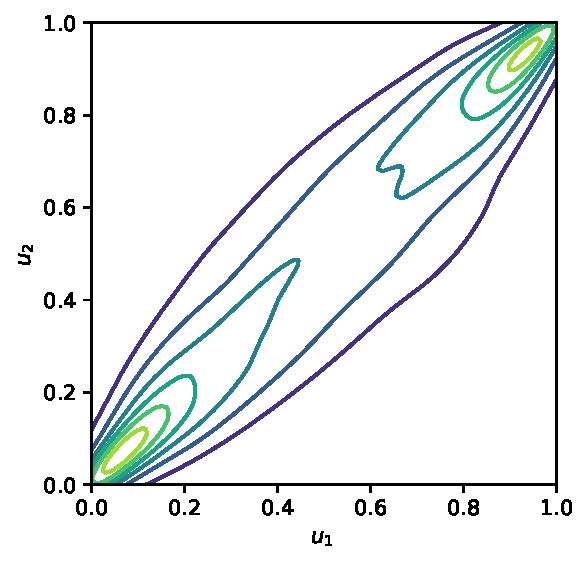
\includegraphics[width = \linewidth]{figures/ND examples/Gaussian copula sample contour.pdf}
            \caption{}
        \end{subfigure}%
        ~
        \begin{subfigure}[t]{0.5\linewidth}
            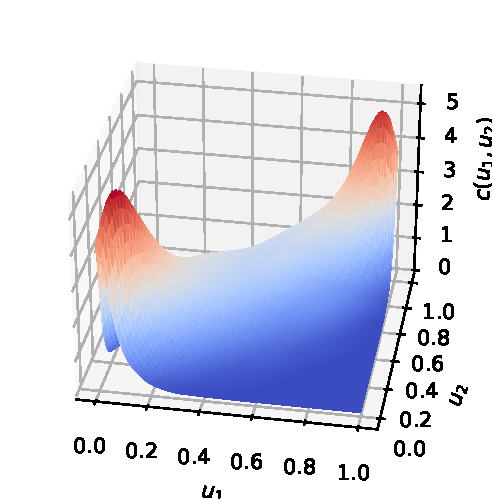
\includegraphics[width = \linewidth]{figures/ND examples/Gaussian copula sample pdf.pdf}
            \caption{}
        \end{subfigure}
        \caption{Estimated copula density $c$ with $\rho = 0.9$ corresponding to $X_1$ and $X_2$.}
        \label{fig:gaussian copula estimate}
    \end{figure}
    The noticeable difference is in the corners $(0,0)$ and $(1,1)$ where the theoretical copula density tends to infinity whereas the estimated density has modes at $(0.1,0.1)$ and $(0.9,0.9)$. In particular, simply rescaling the copula density in \autoref{alg:Gobs1} does not resemble the theoretical boundary which is a known issue \textcolor{red}{reference til artikel om undershoot peaks og boundary conditions for KDE}. A better approach may be to use jackknifing \textcolor{red}{link til afsnit of jackknifing, som også indeholder reference til artikel hvor dette gøres}.
    \begin{figure}[H]
        \centering
        \begin{subfigure}[t]{0.45\linewidth}
            \centering
            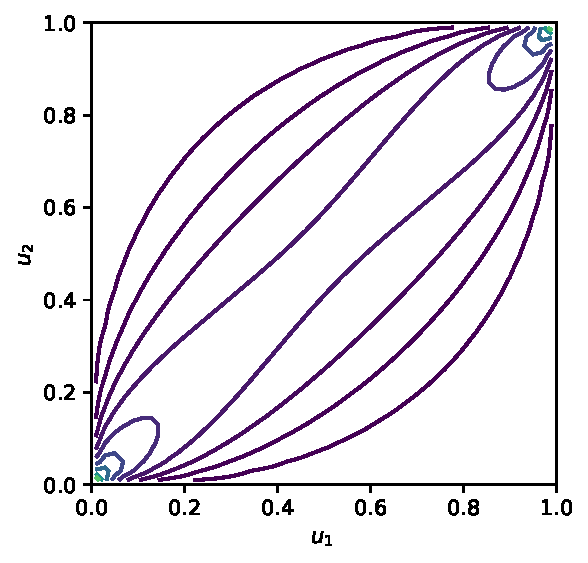
\includegraphics[width = \linewidth]{figures/ND examples/Gaussian copula theoretical contour.pdf}
            \caption{}
        \end{subfigure}%
        ~
        \begin{subfigure}[t]{0.5\linewidth}
            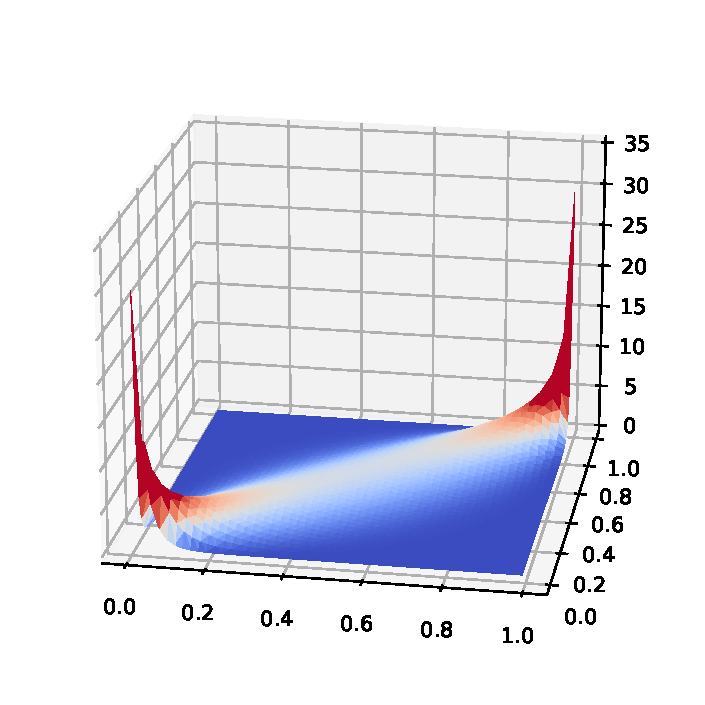
\includegraphics[width = \linewidth]{figures/ND examples/Gaussian copula theoretical pdf.pdf}
            \caption{}
        \end{subfigure}
        \caption{Theoretical copula density $c$ with $\rho = 0.9$ corresponding to $X_1$ and $X_2$.}
        \label{fig:gaussian copula truth}
    \end{figure}
    We note however, that the underlying structure is still captured i.e. that $Y_1$ and $Y_2$ covary while $Y_3$ does not inform $Y_1$ or $Y_2$ and vice versa.
\end{example}

We continue with a similar example to the previous one. The key difference is the number of variables and a more complicated correlation structure to test the algorithms further.
\begin{example}
    From \autoref{ex:1} we saw how one could handle some numerical issues. Thus, in this example we shall not bother ourselves with such computations and merely focus on the correlation structure. In particular, we shall sample $\boldsymbol X$ from a 10 dimensional
\end{example}


\newpage

\section{sammenligning af metoder for at finde MI}
Sammenligning af gammel metode og "min"
\begin{figure}[h]
    \centering
    \begin{subfigure}[t]{0.49\textwidth}
        \centering
        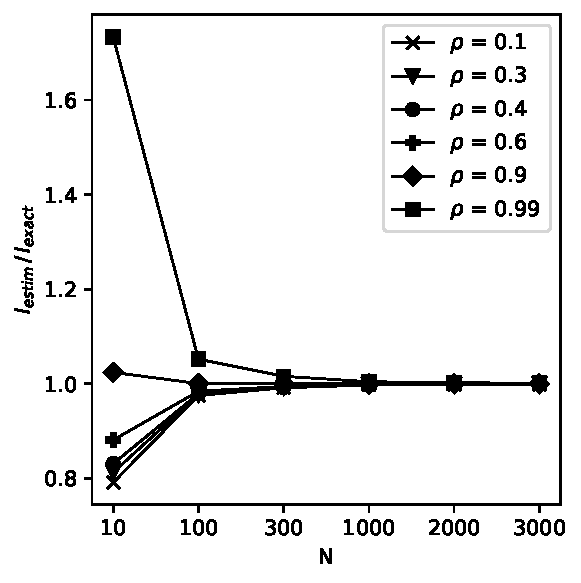
\includegraphics[width=\linewidth]{figures/ND examples/MI calc/gaussian example all.pdf}
        \caption{}
        \label{subfig:new MI method all}
    \end{subfigure}%
    ~
    \begin{subfigure}[t]{0.49\textwidth}
        \centering
        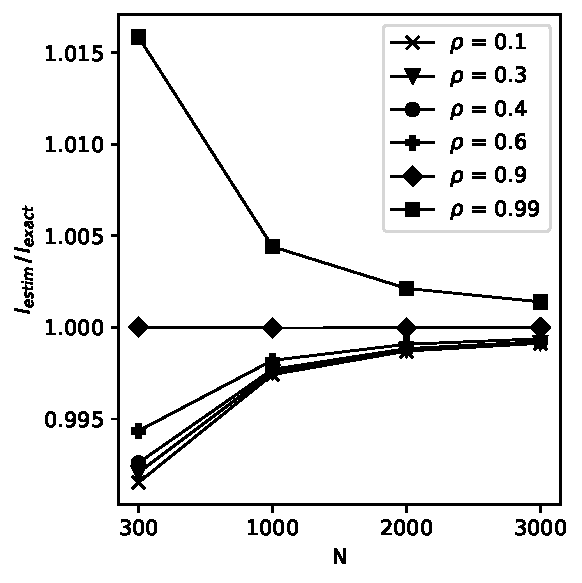
\includegraphics[width=\linewidth]{figures/ND examples/MI calc/gaussian example zoom.pdf}
        \caption{}
        \label{subfig:new MI method all zoom}
    \end{subfigure}
    \caption{Evaluation of MI for new method for different N. \textcolor{red}{Bør sammenlignes med artiekl fundet (har sat i bibtex) og original papers (ikke Kina)}}
    \label{fig:dd}
\end{figure}

\begin{figure}[h]
    \centering
    \begin{subfigure}[t]{0.32\textwidth}
        \centering
        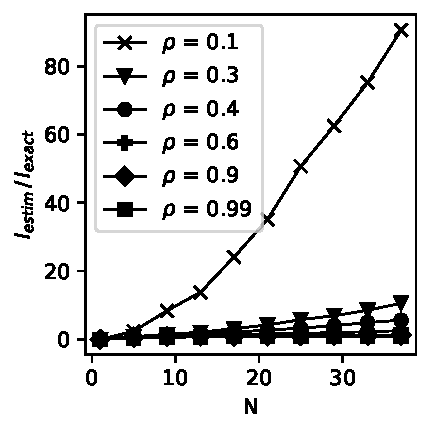
\includegraphics[width=\linewidth]{figures/ND examples/MI calc/gaussian example original all.pdf}
        \caption{}
        \label{subfig:d}
    \end{subfigure}%
    ~
    \begin{subfigure}[t]{0.32\textwidth}
        \centering
        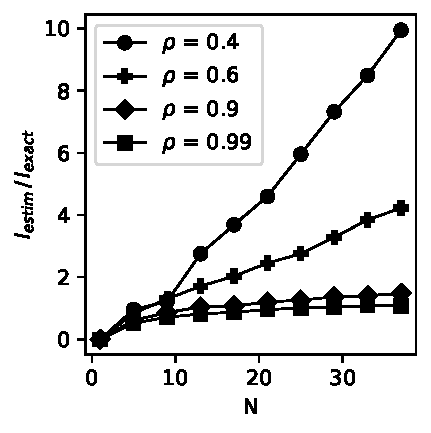
\includegraphics[width=\linewidth]{figures/ND examples/MI calc/gaussian example original zoom.pdf}
        \caption{}
        \label{subfig:dd}
    \end{subfigure}%
    ~
    \begin{subfigure}[t]{0.32\textwidth}
        \centering
        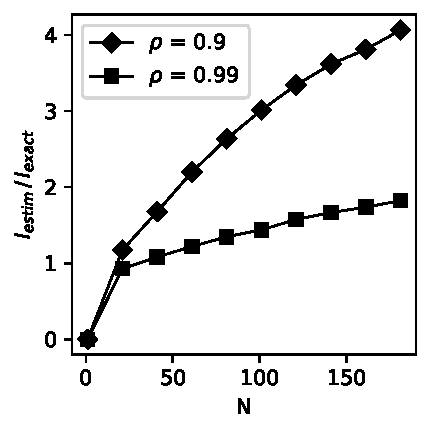
\includegraphics[width=\linewidth]{figures/ND examples/MI calc/gaussian example original high corr.pdf}
        \caption{}
        \label{subfig:ddd}
    \end{subfigure}
    \caption{Evaluation of MI for old method for different N. Ligner der er knæk ved fporhold lig 1. Men ved næremere undersøgelse blev det fundet ud af at det ikke helt er tilfældet, og derudover vil der skulle laves en algoritmisk måde at finde dette knæk på. Savitzky–Golay filter kunne være en mulighed, eller gruppere e.g. 5 forskellige bins og tag gennemsnit. Efter smoothing kan anden afledte tæt på 0 bruges, til at finde hvornår stykket bliver fladt (tilnærmelses vist)}
    \label{fig:ddd}
\end{figure}

\textcolor{red}{ved høj korrelation i.e. tæt på laver dimensionel manifold, skal der bruges mange, som i rigtig mange samples i mesh. }


\textcolor{red}{Inkluder flere exempler end blot gaussian as done by \cite{Estimating-mutual-information-Kraskov}}

\subsection{10D gaussian example}
\textcolor{red}{casuality svarer til at lave nedre/øvre trekant. Er der forskel i at gør edet før og efter for en symmetrisk matrix? - Ja, men begge metoder på 10 eksempel giver gode resultater. Kommenter at det er matematisk meget forskelligt at filtrere først og så ND efter og omvendt}



\end{document}